\chapter{Metodología}
\label{ch:chap3}
% \epigraph{\textit{``Una terrible verdad es mejor que una \'util mentira"}}{--- \textup{Thoman Mann}, La monta\~na m\'agica}

\section{Obtención de locuciones}

En la sección~\ref{sec:sec21} se mencionó que la clave para poder aproximar la estructura lingüística era por medio de una colección de locuciones. Mientras que, en la sección~\ref{sec:sec23} se mencionó que en muchas ocasiones se recurre a las redes sociales para obtener dicha colección. La búsqueda y obtención de locuciones en este trabajo puede resumirse en dos pasos:

\begin{enumerate}
	\item Determinación de las locuciones a buscar
	\item Búsqueda de las locuciones especificadas.
\end{enumerate}

\paragraph{Determinación de las locuciones a buscar.} Al recurrir a las redes sociales, lo primero que debe hacerse es determinar lo que hay que buscar. Para ello, en este trabajo se emplearon los datos proporcionados por \cite{crearae}\footnote{En marzo de 2021 la RAE publica una versión anotada del CREA. Sin embargo contiene una revisión de documentos menos reciente pues solo analiza documentos publicados entre el año 1975 y el año 2000.} que, de cuerdo con Real Academia Española (RAE) consta de una amplía variedad de textos de habla hispana desde 1975 hasta 2004 y una lista de más de 700,000 locuciones del español.

\begin{table}[h]
	\caption{Lista de las 10 palabras más frecuentes en el español de acuerdo con el CREA.}
	\label{tb:creafreq}
	\centering
	\begin{tabular}{|c|c|}
		\hline
		\textbf{Palabra} & \textbf{Frecuencia} \\ \hline
		de               & 9,999,518           \\ \hline
		la               & 6,277,560           \\ \hline
		que              & 4,681,839           \\ \hline
		el               & 4,569,652           \\ \hline
		en               & 4,234,281           \\ \hline
		y                & 4,180,279           \\ \hline
		a                & 3,260,939           \\ \hline
		los              & 2,618,657           \\ \hline
		se               & 2,022,514           \\ \hline
		del              & 1,857,225           \\ \hline
	\end{tabular}
\end{table}

El CREA proporciona la lista de locuciones y la frecuencia de aparición dentro de un conjunto de 140,000 documentos analizados (Tabla~\ref{tb:creafreq}). Sin embargo, en la práctica la inclusión de algunas palabras puede ocasionar efectos no deseados en la estimación de los modelos empleados en el PLN. Para ello, desde el nacimiento del PLN se ha hecho empleo de un conjunto llamado \textit{stop-words} o diccionario negativo el consta de una lista de términos que se excluyen en la estimación del modelo para mejorar los resultados obtenidos en tareas de PLN \citep{fox1989stop}. En el caso del español, el trabajo publicado por \cite{stopwords_es} ha recibido mucha aceptación, por lo que su diccionario negativo de 990 palabras fue el que se empleó para filtrar algunas de las palabras de la lista original del CREA (Tabla~\ref{tb:creafreq_filtered}).

\begin{table}[h]
	\caption{Lista de las 10 palabras más frecuentes en el español de acuerdo con el CREA excluyendo las palabras del diccionario negativo.}
	\label{tb:creafreq_filtered}
	\centering
	\begin{tabular}{|c|c|}
		\hline
		\textbf{Palabra} & \textbf{Frecuencia} \\ \hline
		años             & 203,027             \\ \hline
		vida             & 123,491             \\ \hline
		gobierno         & 113,011             \\ \hline
		país             & 104,568             \\ \hline
		mundo            & 101,745             \\ \hline
		año              & 100,790             \\ \hline
		forma            & 97,165              \\ \hline
		caso             & 96,979              \\ \hline
		millones         & 81,999              \\ \hline
		españa           & 80,195              \\ \hline
	\end{tabular}
\end{table}

\paragraph{Búsqueda de las locuciones especificadas.} La búsqueda, al momento de escribir esta tesis, es tan sencilla como buscar en algo en Google. Sin embargo, para poder llegar a estas alturas fue necesario hacer lo siguiente:
\begin{enumerate}
	\item Configuración del acceso remoto a la red social.
	\item Procesamiento de la información obtenida, que consiste en la descarga, lectura de la información y almacenamiento en legible de la información obtenida.
\end{enumerate}

La mayoría de las redes sociales ofrece un acceso remoto a su red social con el fin de apoyar a sus clientes que usualmente son compañías que buscan alguna interacción con los usuarios del la misma. Para ello, \cite{twitterdev} ofrece una opción para desarrolladores abierta a cualquier persona u organización enfocada a cuatro tareas principales: Oir y analizar, lo cual consiste en proporcionar acceso a las publicaciones públicas de los usuarios de la red social; Publicidad, lo cual consiste en proveer herramientas para manejar campañas publicitarias dentro de la red social; Publicación, lo cuál consiste en ofrecer herramientas el manejo de imagen y publicaciones de instituciones dentro de la red social y; Captación, que en un conjunto de herramientas que permite dirigir usuarios hacia ciertos contenidos\footnote{La cuenta que se empleó en este trabajo fue creada en 2017, época en la cual no hacia falta más que crear una cuenta en la red social y activar la opción de desarrollador. Sin embargo, después del escándalo ocasionado por Cambridge Analytica en 2018, la creación de una cuenta de desarrollador debe tramitarse y esperar autorización.}.

Para el acceso remoto de cualquier servicio en línea, los prestadores del servicio permiten a los desarrolladores interactuar con sus servicios por medio de una API (Application Programming Interface), la cuál sirve como intermediario entre el lenguaje que emplea el desarrollador y los sistemas del provedor. En este trabajo se empleó la biblioteca \textit{tweepy} v3.8 creada por \cite{tweepy} que sirve como un intermediario de fácil uso entre la API de Twitter y Python y posteriormente se empleeo el script \textit{get\_expressions.py} disponible en mi página de GitHub personal (ver \nameref{ch:prefacio}.)  para obtener 100 publicaciones para cada una de las locuciones contenidas en la lista del CREA con una frecuencia superior a 30 y que no estuvieran contenidas en el diccionario negativo. En total 100,337 locuciones fueron buscadas y se obtuvieron en la mayoría de los casos 100 publicaciones donde aparecían éstas. Lo que dio un total de de 10,033,700 de publicaciones obtenidas y procesadas, donde cada publicación cuenta con un promedio de 10 palabras, por lo que en total se formó una colección de aproximadamente 100,337,000 elementos\footnote{La información recabada representa aproximadamente tan solo 1.8 GB de información. Sin embargo, si el lector, desea aventurarse a obtener sus propios ejemplos porque 1.8 GB no es poca información en estos día. Debo advertirle, que debido a que Twitter no permite exceder cierto número de peticiones el tiempo estimado para obtener una colección de este tamaño podría llevarle cerca de 4 meses.}. 

\section{Entrenamiento de las tareas de pre-procesamiento}
Algunas de las tareas de pre-procesamiento necesitan no solo de los ejemplos de uso sino, también requieren de que ese conjunto esté etiquetado. Sin embargo, los conjuntos de datos provenientes de las redes sociales no vienen entrenados. Para ello se empleó lo que se conoce como \textit{Web Scrapping} para automatizar las tareas manuales y debido, a las restricciones impuestas por los servidores de los prestadores de servicio, se recurrió al empleo de la Red Privada Virtual de Kaspersky (VPN, por sus siglas en inglés) para evitar, en medida de lo posible, la interrupción del \textit{Web Scrapping} por una tasa excesiva de peticiones.

\cite{chapagain2019hands} define el \textit{Scrapping} como una serie de tareas que consisten en: extraer, copiar, revisar y/o recolectar información y que, cuando la información procede de la web, entonces se agrega el adjetivo de \textit{Web} a \textit{Scrapping.} En el caso de este trabajo se recurrió a extraer información de la RAE y del sitio \url{http://tulengua.es/silabas} donde está implementado el algoritmo de silabeo propuesto por \cite{hernandez2013automatic} puesto que, una propuesta colateral de este trabajo consistió en la implementación del modelo de la sílaba para ahorrar tiempo en algunas de las tareas.  

Los scripts de scrapping pueden ser igualmente encontrados en el proyecto de GitHub y están contenidos en dos archivos por separado:
\begin{itemize}
	\item \texttt{rae\_scrapping.py}
	\item \texttt{tulengua\_scrapping.py}
\end{itemize}

Ambos archivos realizan la búsqueda automática usando la biblioteca \textit{selenium}\footnote{Para más información sobre le uso de selenium se puede visitar el sitio \url{https://selenium-python.readthedocs.io/}} y extraen el código HTML del resultado y posteriormente se emplean expresiones regulares para extraer la información requerida. En el caso de la RAE, después de una inspección manual del código HTML se determinaron las siguientes expresiones regulares para extraer la información:

\begin{enumerate}
	\item '\textless'+tag\_name+'[\textasciicircum\textgreater]*\textgreater[\textasciicircum\textless\textgreater]\textasciicircum\textless/'+tag\_name+'\textgreater'
	
	\item '\textless'+tag\_name+'[\textasciicircum\textgreater]*\textgreater[\textasciicircum\textless\textgreater]*\textless sup\textgreater'
	
	\item '\textgreater[\textasciicircum\textless]*\textless'
\end{enumerate}

La primera expresión regular permite identificar la etiqueta principal donde se alojan los resultados requeridos que, en este caso son las abreviaturas con las que se determina si una palabra es un sustantivo, verbo, adjetivo, adverbio, etc. La segunda expresión permite identificar la etiqueta principal de algunos casos especiales y la tercera expresión regular se emplean para eliminar el código HTML y dejar solo el resultado deseado en texto plano.

En lo que respecta al segundo sitio, donde se encuentra el algoritmo de silabeo, las expresiones regulares empleados fueron:

\begin{enumerate}
	\item divide\textbackslash s en\textbackslash s[0-9]+\textbackslash ssílabas:\textbackslash s[\textasciicircum.]+
	
	\item :.*
	
	\item \textless/?b\textgreater
	
	\item /[:\textbackslash s]+/
\end{enumerate}

La primera expresión permite identificar donde se arroja el resultado; mientras que las expresiones 2-4 se emplean para limpiar la cadena y dejar el resultado en texto plano.

\section{Algoritmo de silabeo y segmentación}
\label{sec:sec33}

\subsubsection{Algoritmo de silabeo}

Como se mencionó en la sección~\ref{sec:sec25} la mayoría de los algoritmos para el silabeo automático en español son algoritmos basados en reglas. El algoritmo propuesto en este trabajo consiste en que las reglas se puedan reproducir bajo un modelo de una red neuronal.

\begin{figure}[h]
	\centering
	\begin{tikzpicture}[->,>=stealth',auto,semithick,]
		\tikzstyle{every state}=[draw=black,thick,text=black,scale=1]
		\node[state]    (c1)[fill=black!30!green]               				  {$\mathbf{c}_1$};
		\node[state]    (c2)[below of=c1, node distance=1.5cm,fill=black!30!green ]               				  {$\mathbf{c}_2$};
		\node[state]    (c3)[below of=c2, node distance=1.5cm,fill=black!30!green]               				  {$\mathbf{c}_3$};
		\node[state]    (c4)[below of=c3, node distance=1.5cm,fill=black!30!green]               				  {$\mathbf{c}_4$};
		\node[state]    (c5)[below of=c4, node distance=1.5cm,fill=black!30!green]               				  {$\mathbf{c}_5$};
		\node[state]    (h1)[right of=c1, node distance=3cm,fill=white!40!blue]               				  {};
		\node[state]    (h2)[right of=c2, node distance=3cm,fill=white!40!blue]               				  {};
		\node[state]    (h3)[right of=c3, node distance=3cm,fill=white!40!blue]               				  {};
		\node[state]    (h4)[right of=c4, node distance=3cm,fill=white!40!blue]               				  {};
		\node[state]    (h5)[right of=c5, node distance=3cm,fill=white!40!blue]               				  {};
		\node[state]    (y1)[right of=h2, node distance=3cm,fill=white!40!red]               				  {$\mathbf{y}_1$};
		\node[state]    (y2)[right of=h3, node distance=3cm,fill=white!40!red]               				  {$\mathbf{y}_2$};
		\node[state]    (y3)[right of=h4, node distance=3cm,fill=white!40!red]               				  {$\mathbf{y}_3$};
		\path
		(c1) edge (h1)
		(c1) edge (h2)
		(c1) edge (h3)
		(c1) edge (h4)
		(c1) edge (h5)
		(c2) edge (h1)
		(c2) edge (h2)
		(c2) edge (h3)
		(c2) edge (h4)
		(c2) edge (h5)
		(c3) edge (h1)
		(c3) edge (h2)
		(c3) edge (h3)
		(c3) edge (h4)
		(c3) edge (h5)
		(c4) edge (h1)
		(c4) edge (h2)
		(c4) edge (h3)
		(c4) edge (h4)
		(c4) edge (h5)
		(c5) edge (h1)
		(c5) edge (h2)
		(c5) edge (h3)
		(c5) edge (h4)
		(c5) edge (h5)
		(h1) edge (y1)
		(h1) edge (y2)
		(h1) edge (y3)
		(h2) edge (y1)
		(h2) edge (y2)
		(h2) edge (y3)
		(h3) edge (y1)
		(h3) edge (y2)
		(h3) edge (y3)
		(h4) edge (y1)
		(h4) edge (y2)
		(h4) edge (y3)
		(h5) edge (y1)
		(h5) edge (y2)
		(h5) edge (y3);
	\end{tikzpicture}
	\caption{Arquitectura propuesta para el modelo de red neuronal que será el núcleo de la silabeo automático.}
	\label{fig:syllabification}
\end{figure}

La Fig.~\ref{fig:syllabification} propone que el algoritmo emplee el hecho de que una sílaba en español no puede exceder los 5 caracteres. En ese sentido, las entradas del modelo $c_i$ son, son un conjunto de 5 caracteres donde al menos uno de los caracteres es una vocal. Las salidas $y_i$ obedecen a las probabilidades de que la separación silábica ocurra en la i-ésima posición del bloque. Note que el modelo emula la arquitectura CBOW con la intención que en la capa oculta se condensen las relaciones de los caracteres. Así, en un principio las funciones de activación asociadas a cada capa son las mismas que las empleadas por Mikolov en el modelo CBOW. De esta forma el algoritmo de silabeo propuesto es el siguiente:

\begin{megaalgorithm}
	\caption{Algoritmo de Silabeo}
	\label{alg:syllabification}
	\begin{algorithmic}[1]
		\Procedure{Syllabification}{$w$}\Comment{w es una palabra}
		\State $syllables\gets []$
		\State $position\gets 0$
		\State $wc\gets \mbox{\textsc{codification}}(w)$
		\While{$postion < len(wc)$}
		\State $block\gets wc[0:5]$
		\State $cut\gets \mbox{\textsc{core\_syllabification}}(block)$
		\State $syllables\gets \mbox{\textsc{add}}(syllables,wc[position:(position+cut)])$
		\State $position\gets position + cut$
		\EndWhile
		\State \textbf{return} $syllables$
		\EndProcedure
	\end{algorithmic}
\end{megaalgorithm}
donde el procedimiento \textsc{codification} corresponde a una función de codificación que asigna a cada carácter un valor de acuerdo con la Tabla~\ref{tb:codsound} y el procedimiento \textsc{core\_syllabification} corresponde a la aplicación del modelo de red neuronal descrito en la Fig.~\ref{fig:syllabification}. 

\begin{table}[H]
	\centering
	\caption{Tabla reducida de los sonidos del español con base en la obra de \cite{hualde2013sonidos}.}
	\label{tb:codsound}
\begin{tabular}{|c|c|c|c|}
	\hline
	\textbf{Modo} & \textbf{Marca} & \textbf{Símbolo} & \textbf{Grupo} \\ \hline
	\multicolumn{2}{|c|}{Sin sonido}                                                   & h /\textipa{2}/  & 0                               \\ \hline
	Oclusivo                                & Bilabial                                 & p b v                             & 1                               \\ \hline
	Oclusivo                                & Dental                                   & t d                               & 1                               \\ \hline
	Oclusivo                                & Velar                                    & k q g                             & 2                               \\ \hline
	Fricativo                               & Labiodental                              & f                                 & 3                               \\ \hline
	Fricativo                               & Alveolar                                 & s z                               & 4                               \\ \hline
	Fricativo                               & Palatal                                  & y ll                              & 4                               \\ \hline
	Fricativo                               & Velar                                    & j g x                             & 5                               \\ \hline
	Africado                                & Palatal                                  & ch                                & 6                               \\ \hline
	Nasal                                   & Bilabial                                 & m                                 & 7                               \\ \hline
	Nasal                                   & Alveolar                                 & n                                 & 8                               \\ \hline
	Nasal                                   & Palatal                                  & ñ                                 & 8                               \\ \hline
	Aproximante Lateral                     & Alveolar                                 & l                                 & 9                               \\ \hline
	Percusivo                               & Alveolar                                 & r                                 & 10                              \\ \hline
	Vibrante                                & Alveolar                                 & r rr                              & 10                              \\ \hline
	\multicolumn{2}{|c|}{Vocal fuerte}                                                 & a e o                             & 11                              \\ \hline
	\multicolumn{2}{|c|}{Vocal débil}                                                  & i u                               & 12                              \\ \hline
	\multicolumn{2}{|c|}{Semi-vocal}                                                   & w gü                              & 13                              \\ \hline
\end{tabular}
\end{table}

Además, los scripts de procesamiento, entrenamiento, validación e implementación se pueden encontrar en los siguientes archivos del proyecto de GitHub:

\begin{itemize}
	\item \texttt{syllabification\_code.py} Script que se encarga de la codificación básica con base en la Tabla .
	\item \texttt{syllabification\_train.py} Script que se encarga del entrenamiento de lo que representa el \textsc{core\_syllabification}. El entrenamiento se realizó usando Keras y Tensorflow.
	\item \texttt{sil\_test.py} Script que se encarga de decodificar la información proporcionada por el \textsc{core\_syllabification}.
	\item \texttt{sil\_compare.py} Script que se encarga de la realización de las pruebas de validación, comparando los resultados del método propuesto por \cite{hernandez2013automatic} y el propuesto en este trabajo.
	\item \texttt{sil\_model.json} Archivo que contiene la arquitectura del modelo de red neuronal para su rápida carga usando Keras.
	\item \texttt{sil\_weights.h5} Archivo que contiene los pesos del modelo de la red neuronal para su uso futuro.
	\item \texttt{sil\_xtrain.np} Datos codificados para entrenamiento.
	\item \texttt{sil\_ytrain.np} Datos codificados para entrenamiento.
	\item \texttt{syllables\_dataset.json} Dados en bruto para entrenamiento.
\end{itemize}

\subsection{Algoritmo de segmentación}

\cite{cano2019segmentacion} menciona que el proceso de optimización planteado por (\ref{eq:norvig}) puede ser computacionalmente extensivo cuando se emplean 2-gramas. Sin embargo, también menciona que el método de 2-gramas es mejor que el enfoque más sencillo planteado al usar 1-gramas. En ese sentido, se propone lo siguiente:

\begin{itemize}
	\item Los cortes en una gran mayoría de los casos aparecen al final de una sílaba\footnote{Usualmente ocurre así. aunque dar por hecho esto puede llevar a errores sistemáticos. Por ejemplo, uno de los \textit{hashtags} de prueba empleados por \cite{cano2019segmentacion} fue ``DíaInternacionaldelamujer'' y el silabeo correcto esta dado por \textit{dí-\textbf{ain}-ter-na-ci-o-nal-de-la-mu-jer}. Note que la separación correcta ocurre entre la sílaba en negritas, lo que implica su imposible separación.}. Del conjunto empleado por \cite{cano2019segmentacion} solo el 3\% de los \textit{hashtags} no cumplen esa característica.
	
	\item \cite{gai2014bidirectional} proponen que en la optimización de (\ref{eq:norvig}) puede hacerse al generar una segmentación en dos direcciones. Por ejemplo, para separar ``elchistedelnorte'' la optimización hacia adelante, que es la empleada por Norvig, evalúa a los candidatos \textit{e}, \textit{el}, \textit{elc}, etc. Sin embargo, el proceso puede hacerse hacia atrás donde se evalúan los candidatos \textit{e}, \textit{te}, \textit{rte},etc.
	
	\item Al dividir la cadena en dos subcadenas disjuntas aleatorias es probable que haya al menos una palabra en alguno de las dos subcadenas obtenidas.
\end{itemize}

El algoritmo de segmentación propuesto y empleado en este consiste en la combinación los tres elementos antes mencionados. Los algoritmos base se describen a continuación y pueden encontrarse condensados en el archivo \texttt{segmentation.py}.

\begin{megaalgorithm}[h]
	\caption{Algoritmo de Segmentación}
	\label{alg:segmentation}
	\begin{algorithmic}[1]
		\Procedure{Segmentation}{$s$}\Comment{s es una cadena}
		\State $blocks\gets \mbox{\textsc{syllabification}}(s)$
		\State $k\gets \mbox{\textsc{randomint}}(0,n)$ \Comment{n es el número de sílabas de s}
		\State $b_1,b_2\gets blocks[0:k],blocks[k:n]$
		\State $c_{b1A},c_{b1B}\gets \mbox{\textsc{segmentation\_foward}}(b_1),\mbox{\textsc{segmentation\_backward}}(b_1)$
		\State $c_{b2A},c_{b2B}\gets \mbox{\textsc{segmentation\_foward}}(b_2),\mbox{\textsc{segmentation\_backward}}(b_2)$
		\State $candidates\gets \mbox{\textsc{mix}}(c_{b1A},c_{b1B},c_{b2A},c_{b2B})$
		\State $s_split\gets \mbox{\textsc{optimize}}(candidates)$
		\State \textbf{return} $s_split$
		\EndProcedure
	\end{algorithmic}
\end{megaalgorithm}

\begin{megaalgorithm}[h]
	\caption{Algoritmo de Segmentación hacia adelante}
	\begin{algorithmic}[1]
		\Procedure{Segmentation\_foward}{$b$}\Comment{b es una lista de sílabas}
		\State $condition\gets TRUE$
		\State $k\gets 1$
		\State $P_0\gets \mbox{\textsc{probability}}(b)$
		\State $split_b \gets []$
		\While{condition = TRUE \mbox{\textbf{\textsc{and}}} len(b) \textgreater k}
		\State $A_c, A_r \gets b[0:k],b[k:]$
		\State $B_c, B_r \gets b[0:(k+1)],b[(k+1):]$
		\State $P_A \gets \mbox{\textsc{probability}}(A_c) \times \mbox{\textsc{probability}}(A_r)$
		\State $P_B \gets \mbox{\textsc{probability}}(B_c) \times \mbox{\textsc{probability}}(B_r)$
		\State $condition \gets P_B < P_A$
		\If{condition = FALSE \mbox{\textbf{\textsc{and}}} $P_B > P_0$}
		\State $\mbox{\textsc{add}}(split_b, B_c)$
		\ElsIf{condition = FALSE \mbox{\textbf{\textsc{and}}} $P_B < P_0$}
		\State $\mbox{\textsc{add}}(split_b, b)$
		\EndIf
		\State $k \gets k+1$
		\EndWhile
		\State \textbf{return} $split_b$
		\EndProcedure
	\end{algorithmic}
\end{megaalgorithm}

\begin{megaalgorithm}[h]
	\caption{Algoritmo de Segmentación hacia atras}
	\begin{algorithmic}[1]
		\Procedure{Segmentation\_foward}{$b$}\Comment{b es una lista de sílabas}
		\State $condition\gets TRUE$
		\State $k\gets n-1$ \Comment{n es el número de elementos de b}
		\State $P_0\gets \mbox{\textsc{probability}}(b)$
		\State $split_b \gets []$
		\While{condition = TRUE \mbox{\textbf{\textsc{and}}} 0 \textgreater k}
		\State $A_c, A_r \gets b[k:],b[:k]$
		\State $B_c, B_r \gets b[(k-1):],b[:(k-1)]$
		\State $P_A \gets \mbox{\textsc{probability}}(A_c) \times \mbox{\textsc{probability}}(A_r)$
		\State $P_B \gets \mbox{\textsc{probability}}(B_c) \times \mbox{\textsc{probability}}(B_r)$
		\State $condition \gets P_B < P_A$
		\If{condition = FALSE \mbox{\textbf{\textsc{and}}} $P_B > P_0$}
		\State $\mbox{\textsc{add}}(split_b, B_c)$
		\ElsIf{condition = FALSE \mbox{\textbf{\textsc{and}}} $P_B < P_0$}
		\State $\mbox{\textsc{add}}(split_b, b)$
		\EndIf
		\State $k \gets k-1$
		\EndWhile
		\State \textbf{return} $split_b$
		\EndProcedure
	\end{algorithmic}
\end{megaalgorithm}

Note que los algoritmos requieren un cálculo de probabilidad, probabilidad que calcula con base en las frecuencias relativas de las palabras si la palabra es conocida y usando (\ref{eq:norvigunknown}) si la palabra es desconocida. Además, la probabilidad se requiere que los bloques estén concatenados previamente, lo cual se omite dentro de los algoritmos para facilitar su lectura. Por otro lado, las funciones \textsc{mix} y \textsc{optimize} involucradas en el Alg.~\ref{alg:segmentation} no se describen a detalle porque, en el caso de la primera consiste en generar las combinaciones que se generan de por medio de los algoritmos de segmentación y, la segunda consiste en seleccionar aquella combinación con probabilidad mayor. La razón es también que sea sencilla la lectura.
  
\section{Pre-procesamiento de la locuciones}

Para ilustrar la aplicación de los métodos discutidos en el capítulo anterior se tomará de ejemplo algunas de las publicaciones obtenidas para una palabra específica. 

\paragraph{Texto bruto.} La Fig.~\ref{fig:tweets_raw} muestra como se ven algunos de publicaciones obtenidas\footnote{Por cada palabra se generaron 10 archivos, y no existe una justificación técnica al respecto de porque se prefirió generar 10 archivos por palabra en lugar de uno. Esto obedeció a que se prefirió tener algunos ejemplos de todas las palabras para comenzar a explorar.}, donde cada publicación se encuentra separada por una cadena compuesta por exactamente 10 símbolos de porcentaje.

\begin{figure}[h]
	\centering
	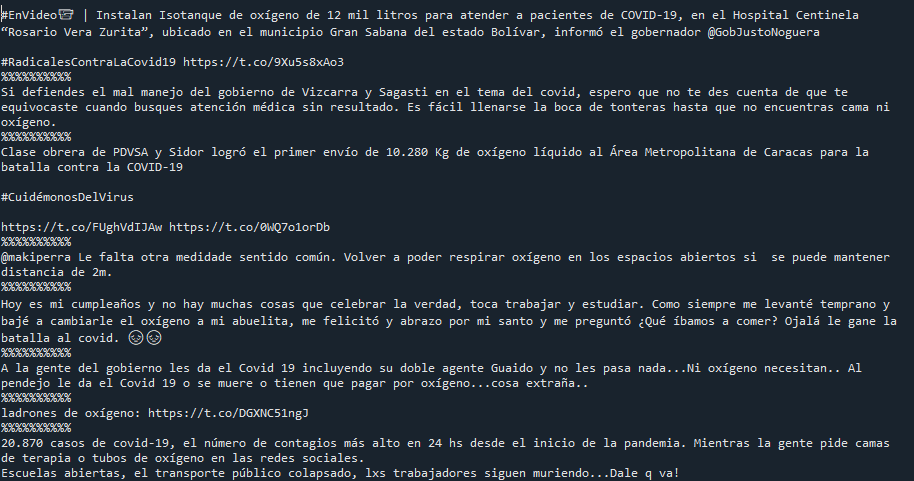
\includegraphics[width=0.95\linewidth]{img/tweets_raw}
	\caption{Imagen que muestra algunas de las publicaciones en bruto sobre la palabra ``oxígeno''. Se muestra en imagen porque algunos caracteres no son manejables en \LaTeX.}
	\label{fig:tweets_raw}
\end{figure}

\paragraph{Separación.} La separación consiste en en segmentar el texto completo en una lista de elementos donde cada elemento sea una publicación, luego separar las en palabras tentativas cada publicación. A continuación se muestran los \textit{tweets} de la Fig~\ref{fig:tweets_raw} después de la separación donde se resaltan los términos problemáticas en rojo\footnote{Pudiera parecer sorprendente que términos como \textit{psvsa} hayan sido reconocidos, pero en efecto forman parte del CREA.}; mientras que en azul se resultan los términos poco frecuentes:

\begin{quote}
	\textcolor{red}{}Instalan \textcolor{red}{Isotanque} de oxígeno de \textcolor{red}{12} mil litros para atender a pacientes de \textcolor{red}{COVID} \textcolor{red}{19} en el Hospital Centinela Rosario Vera Zurita ubicado en el municipio Gran Sabana del estado Bolívar informó el gobernador \textcolor{red}{@GobJustoNoguera} \textcolor{red}{\#RadicalesContraLaCovid19} \textcolor{red}{} 
	\vspace{12pt} \\
	\textcolor{red}{}Si defiendes el mal manejo del gobierno de \textcolor{blue}{Vizcarra} y Sagasti en el tema del \textcolor{red}{covid} espero que no te des cuenta de que te equivocaste cuando busques atención médica sin resultado Es fácil llenarse la boca de \textcolor{blue}{tonteras} hasta que no encuentras cama ni oxígeno \textcolor{red}{} 
	\vspace{12pt} \\
	\textcolor{red}{}Clase obrera de PDVSA y Sidor logró el primer envío de \textcolor{red}{10} \textcolor{red}{280} Kg de oxígeno líquido al Área Metropolitana de Caracas para la batalla contra la \textcolor{red}{COVID} \textcolor{red}{19} \textcolor{red}{\#CuidémonosDelVirus} \textcolor{red}{} 
	\vspace{12pt} \\
	\textcolor{red}{}\textcolor{red}{@makiperra} Le falta otra \textcolor{red}{medidade} sentido común Volver a poder respirar oxígeno en los espacios abiertos si se puede mantener distancia de \textcolor{red}{2m} \textcolor{red}{} 
	\vspace{12pt} \\
	\textcolor{red}{}Hoy es mi cumpleaños y no hay muchas cosas que celebrar la verdad toca trabajar y estudiar Como siempre me levanté temprano y bajé a cambiarle el oxígeno a mi abuelita me felicitó y abrazo por mi santo y me preguntó Qué íbamos a comer Ojalá le gane la batalla al \textcolor{red}{covid} \textcolor{red}{} 
	\vspace{12pt} \\
	\textcolor{red}{}A la gente del gobierno les da el \textcolor{red}{Covid} \textcolor{red}{19} incluyendo su doble agente \textcolor{red}{Guaido} y no les pasa nada Ni oxígeno necesitan Al pendejo le da el \textcolor{red}{Covid} \textcolor{red}{19} o se muere o tienen que pagar por oxígeno cosa extraña \textcolor{red}{} 
	\vspace{12pt} \\
	\textcolor{red}{}ladrones de oxígeno \textcolor{red}{} 
	\vspace{12pt} \\
	\textcolor{red}{}\textcolor{red}{20} \textcolor{red}{870} casos de \textcolor{red}{covid} \textcolor{red}{19} el número de contagios más alto en \textcolor{red}{24} hs desde el inicio de la pandemia Mientras la gente pide camas de terapia o tubos de oxígeno en las redes sociales Escuelas abiertas el transporte público colapsado \textcolor{red}{lxs} trabajadores siguen muriendo Dale q va \textcolor{red}{} 
	\vspace{12pt} \\
	\textcolor{red}{} \textcolor{red}{@canarias7} Sanidad los expertos que no existen y la madre que los parió a todos El oxígeno gratuito y es de todos quienes se creen dueños para permitir si respiramos o no en nuestro descanso y más en la playa o el campo \textcolor{red}{} 
	\vspace{12pt} \\
	\textcolor{red}{}\textcolor{red}{@abc} es Desobediencia civil y no hacer caso de un gobierno corrupto con conflicto de intereses en la venta de mascarillas No al bozal mi vida mi oxígeno Prohibición de mascarilla al aire libre ya \textcolor{red}{} 
\end{quote}

\paragraph{Segmentación.} La segmentación emplea los algoritmos descritos en la sección~\ref{sec:sec33}. La aplicación lleva a obtener lo siguiente:

\begin{quote}
	Instalan \textcolor{red}{Isotanque} de oxígeno de \textcolor{red}{12} mil litros para atender a pacientes de \textcolor{red}{COVID19} en el Hospital Centinela Rosario Vera Zurita ubicado en el municipio Gran Sabana del estado Bolívar informó el gobernador \textcolor{red}{@GobJustoNoguera} radicales contra la \textcolor{red}{covid19} 
	\vspace{12pt} \\
	Si defiendes el mal manejo del gobierno de \textcolor{blue}{Vizcarra} y Sagasti en el tema del \textcolor{red}{covid} espero que no te des cuenta de que te equivocaste cuando busques atención médica sin resultado Es fácil llenarse la boca de \textcolor{blue}{tonteras} hasta que no encuentras cama ni oxígeno 
	\vspace{12pt} \\
	Clase obrera de PDVSA y Sidor logró el primer envío de \textcolor{red}{10280} Kg de oxígeno líquido al Área Metropolitana de Caracas para la batalla contra la \textcolor{red}{COVID19} \textcolor{blue}{cuidémonos} del virus 
	\vspace{12pt} \\
	\textcolor{red}{@makiperra} Le falta otra \textcolor{red}{medidade} sentido común Volver a poder respirar oxígeno en los espacios abiertos si se puede mantener distancia de \textcolor{red}{2m} 
	\vspace{12pt} \\
	Hoy es mi cumpleaños y no hay muchas cosas que celebrar la verdad toca trabajar y estudiar Como siempre me levanté temprano y bajé a cambiarle el oxígeno a mi abuelita me felicitó y abrazo por mi santo y me preguntó Qué íbamos a comer Ojalá le gane la batalla al \textcolor{red}{covid} 
	\vspace{12pt} \\
	A la gente del gobierno les da el \textcolor{red}{Covid19} incluyendo su doble agente \textcolor{red}{Guaido} y no les pasa nada Ni oxígeno necesitan Al pendejo le da el \textcolor{red}{Covid19} o se muere o tienen que pagar por oxígeno cosa extraña 
	\vspace{12pt} \\
	ladrones de oxígeno 
	\vspace{12pt} \\
	\textcolor{red}{20870} casos de \textcolor{red}{covid19} el número de contagios más alto en \textcolor{red}{24} hs desde el inicio de la pandemia Mientras la gente pide camas de terapia o tubos de oxígeno en las redes sociales Escuelas abiertas el transporte público colapsado \textcolor{red}{lxs} trabajadores siguen muriendo Dale q va 
	\vspace{12pt} \\
	\textcolor{red}{@canarias7} Sanidad los expertos que no existen y la madre que los parió a todos El oxígeno gratuito y es de todos quienes se creen dueños para permitir si respiramos o no en nuestro descanso y más en la playa o el campo 
	\vspace{12pt} \\
	\textcolor{red}{@abc} es Desobediencia civil y no hacer caso de un gobierno corrupto con conflicto de intereses en la venta de mascarillas No al bozal mi vida mi oxígeno Prohibición de mascarilla al aire libre ya 
\end{quote}

\paragraph{PoS y NER.} Las tareas de PoS y NER fueron realizadas usando el Stanford CoreNLP \textit{v4.2}. Los modelos desarrollados por la Universidad de Stanford pueden usarse para realizar un pre-procesamiento completo en inglés y ofrece soporte parcial de algunas tareas para Árabe, Chino, Fránces, Alemán y Español \citep{manning2014stanford}.

\paragraph{Lematizado.}

\section{Estimación del modelo}










